%%%%%%%%%%%%%%%%%%%%%%%%%%%%%%%%%%%%%%%%%
% Arsclassica Article
% LaTeX Template
% Version 1.1 (10/6/14)
%
% This template has been downloaded from:
% http://www.LaTeXTemplates.com
%
% Original author:
% Lorenzo Pantieri (http://www.lorenzopantieri.net) with extensive modifications by:
% Vel (vel@latextemplates.com)
%
% License:
% CC BY-NC-SA 3.0 (http://creativecommons.org/licenses/by-nc-sa/3.0/)
%
%%%%%%%%%%%%%%%%%%%%%%%%%%%%%%%%%%%%%%%%%

%----------------------------------------------------------------------------------------
%	PACKAGES AND OTHER DOCUMENT CONFIGURATIONS
%----------------------------------------------------------------------------------------

\documentclass[
10pt, % Main document font size
a4paper, % Paper type, use 'letterpaper' for US Letter paper
oneside, % One page layout (no page indentation)
%twoside, % Two page layout (page indentation for binding and different headers)
headinclude,footinclude, % Extra spacing for the header and footer
BCOR5mm, % Binding correction
]{scrartcl}

%%%%%%%%%%%%%%%%%%%%%%%%%%%%%%%%%%%%%%%%%
% Arsclassica Article
% Structure Specification File
%
% This file has been downloaded from:
% http://www.LaTeXTemplates.com
%
% Original author:
% Lorenzo Pantieri (http://www.lorenzopantieri.net) with extensive modifications by:
% Vel (vel@latextemplates.com)
%
% License:
% CC BY-NC-SA 3.0 (http://creativecommons.org/licenses/by-nc-sa/3.0/)
%
%%%%%%%%%%%%%%%%%%%%%%%%%%%%%%%%%%%%%%%%%

%----------------------------------------------------------------------------------------
%	REQUIRED PACKAGES
%----------------------------------------------------------------------------------------

\usepackage[
nochapters, % Turn off chapters since this is an article        
beramono, % Use the Bera Mono font for monospaced text (\texttt)
eulermath,% Use the Euler font for mathematics
pdfspacing, % Makes use of pdftex’ letter spacing capabilities via the microtype package
dottedtoc % Dotted lines leading to the page numbers in the table of contents
]{classicthesis} % The layout is based on the Classic Thesis style

\usepackage{arsclassica} % Modifies the Classic Thesis package

\usepackage[T1]{fontenc} % Use 8-bit encoding that has 256 glyphs

\usepackage[utf8]{inputenc} % Required for including letters with accents

\usepackage{graphicx} % Required for including images
\graphicspath{{Figures/}} % Set the default folder for images

\usepackage{enumitem} % Required for manipulating the whitespace between and within lists

\usepackage{lipsum} % Used for inserting dummy 'Lorem ipsum' text into the template

\usepackage{subfig} % Required for creating figures with multiple parts (subfigures)

\usepackage{amsmath,amssymb,amsthm} % For including math equations, theorems, symbols, etc

\usepackage{varioref} % More descriptive referencing

%----------------------------------------------------------------------------------------
%	THEOREM STYLES
%---------------------------------------------------------------------------------------

\theoremstyle{definition} % Define theorem styles here based on the definition style (used for definitions and examples)
\newtheorem{definition}{Definition}

\theoremstyle{plain} % Define theorem styles here based on the plain style (used for theorems, lemmas, propositions)
\newtheorem{theorem}{Theorem}

\theoremstyle{remark} % Define theorem styles here based on the remark style (used for remarks and notes)

%----------------------------------------------------------------------------------------
%	HYPERLINKS
%---------------------------------------------------------------------------------------

\hypersetup{
%draft, % Uncomment to remove all links (useful for printing in black and white)
colorlinks=true, breaklinks=true, bookmarks=true,bookmarksnumbered,
urlcolor=webbrown, linkcolor=RoyalBlue, citecolor=webgreen, % Link colors
pdftitle={}, % PDF title
pdfauthor={\textcopyright}, % PDF Author
pdfsubject={}, % PDF Subject
pdfkeywords={}, % PDF Keywords
pdfcreator={pdfLaTeX}, % PDF Creator
pdfproducer={LaTeX with hyperref and ClassicThesis} % PDF producer
} % Include the structure.tex file which specified the document structure and layout

\hyphenation{Fortran hy-phen-ation} % Specify custom hyphenation points in words with dashes where you would like hyphenation to occur, or alternatively, don't put any dashes in a word to stop hyphenation altogether

\usepackage{listings}
\usepackage[english]{babel}
\selectlanguage{english}

%----------------------------------------------------------------------------------------
%	TITLE AND AUTHOR(S)
%----------------------------------------------------------------------------------------

\title{\normalfont\spacedallcaps{Multiagent team for playing SoccerBots inspired by wasp like task allocation}} % The article title

\author{\spacedlowsmallcaps{Ángel Panizo LLedot\textsuperscript{1}}} % The article author(s) - author affiliations need to be specified in the AUTHOR AFFILIATIONS block

\date{} % An optional date to appear under the author(s)

%----------------------------------------------------------------------------------------

\begin{document}

%----------------------------------------------------------------------------------------
%	HEADERS
%----------------------------------------------------------------------------------------

\renewcommand{\sectionmark}[1]{\markright{\spacedlowsmallcaps{#1}}} % The header for all pages (oneside) or for even pages (twoside)
%\renewcommand{\subsectionmark}[1]{\markright{\thesubsection~#1}} % Uncomment when using the twoside option - this modifies the header on odd pages
\lehead{\mbox{\llap{\small\thepage\kern1em\color{halfgray} \vline}\color{halfgray}\hspace{0.5em}\rightmark\hfil}} % The header style

\pagestyle{scrheadings} % Enable the headers specified in this block

%----------------------------------------------------------------------------------------
%	TABLE OF CONTENTS & LISTS OF FIGURES AND TABLES
%----------------------------------------------------------------------------------------

\maketitle % Print the title/author/date block

\setcounter{tocdepth}{2} % Set the depth of the table of contents to show sections and subsections only

\tableofcontents % Print the table of contents

\listoffigures % Print the list of figures

%----------------------------------------------------------------------------------------
%	ABSTRACT
%----------------------------------------------------------------------------------------
\newpage

\section*{Abstract} % This section will not appear in the table of contents due to the star (\section*)

In this paper a multiagent system inspired on wasp like task allocation capable of playing SoccerBots\footnote{http://www.cs.cmu.edu/~trb/TeamBots/Domains/SoccerBots/} is presented. The several stimulus and actions that they trigger will be described. The performance of this approach will be tested against the teams made for SBTournament\footnote{http://gaia.fdi.ucm.es/research/sbtournament} by students of the Complutense University of Madrid.    

%----------------------------------------------------------------------------------------
%	AUTHOR AFFILIATIONS
%----------------------------------------------------------------------------------------

{\let\thefootnote\relax\footnotetext{\textsuperscript{1} \textit{Agentes inteligentes y sistemas multiagente, Universidad Politécnica de Madrid, Madrid, España}}}

%----------------------------------------------------------------------------------------

\newpage % Start the article content on the second page, remove this if you have a longer abstract that goes onto the second page

%----------------------------------------------------------------------------------------
%	INTRODUCTION
%----------------------------------------------------------------------------------------

\section{Introduction}

\begin{figure}
	\centering
	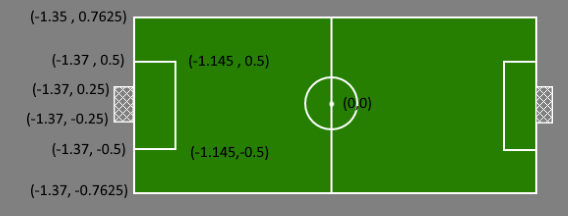
\includegraphics[width=1\linewidth]{campo}
	\caption{Dimensions of the field}
	\label{fig:fig}
\end{figure}

We proposed a team of SoccerBots based on a multiagent approach, where each agent is inspired by the wasps  behavior allocating tasks and Bonabeau model\cite{bonabeau1997adaptive}. Each agent has its own threshold, when a stimuli is bigger than the corresponding threshold the agent does an action in response that stimuli. For example the emptier and nearer the opponent's goal is, from certain player perspective, the bigger the stimuli for shooting. When the corresponding threshold, unique for that agent, is exceeded the agent shoots.\\

SoccerBots simulates the dynamics and dimensions of a regulation RoboCup\footnote{https://www.sonycsl.co.jp/person/kitano/RoboCup/RoboCup.html} small size robot league game, which have 5 players in each team and the dimensions of the field is 152.5cm by 274cm. Each goal is 50cm wide. The *goalkeeper area*, centered on the goal, is 100cm wide by 22.5cm deep. In the coordinate system used in the simulation, the *center of the field* is (0,0) with +x to the right (east) and +y up (north). The team that starts on the left side (or *west field*) is called the *west team* and the team on the right (or *east field*) is called the *east team*. The following schema sketches the main points for the west field (coordinates are in meters). See figure 1.\\

On top of that the software SBTournament is used which enhanced the SoccerBots and has teams implemented by students of the UCM\footnote{Universidad Complutense de Madrid}. These teams will be used to evaluated the efficiency of the multiagent team proposed in this paper.\\ 

Other works in this area are: \cite{wu2004fuzzy} which implements a team using fuzzy rules, \cite{shi2015research} where a self-adaptive method is proposed and \cite{ros2009case} where a case-based approach is used from which this paper is inspired.\\

The paper is structured as following: in section 2 the different stimulus which the agent receive are described, in section 3 the territorial division of the field is explained, in section 4 the actions and threshold available for an agent, in section 5 the method for adjusting the threshold, section 6 the result obtained compared to the teams available in SBTournament and finally in section 7 the conclusions and future work.  

%----------------------------------------------------------------------------------------
%	Territorial task division
%----------------------------------------------------------------------------------------

\section{Territorial task division}

\begin{figure}
	\centering
	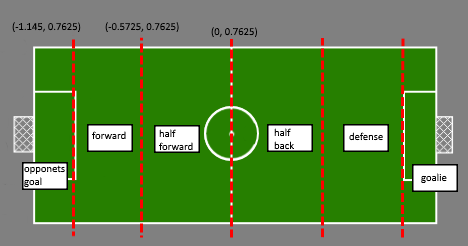
\includegraphics[width=0.7\linewidth]{territorio}
	\caption{Territories}
	\label{fig:fig}
\end{figure}

Inspired by \cite{baghaei2007multi} territorial task division the soccer field was divided into six
territories, namely: goalie, defense, halfback, half-forward, forward and opponent's goal. These territories are shown in Figure 2. The total workspace is rectangular area that is bounded by $(x_{min}, y_{min})$ and $(x_{max}, y_{max})$. All the workspaces were assigned the same length, which was $|Y_{max} - Y_{min}|$ and the Xs as the Figure 2 shows. These divisions enables the team players to be more distributed and interfere   less between each other.  
 
%----------------------------------------------------------------------------------------
%	Stimulus
%----------------------------------------------------------------------------------------

\section{Stimulus}
The several stimulus the agent will react to are the: score and remaining time, the defense,
competition and angle factors defined in \cite{wu2004fuzzy}  and the: situation, cover and penetration(some changes were made from the original) factors defined in \cite{shi2015research} and finally the: shooting and keep goal factors of my own invention. Therefore, their definitions will first be given in this section. All stimulus are functions between 0 and 1.

\subsection{Score}
This stimuli is the score of the match, 1 if our team is winning by much advantage and 0 if it is losing. The stimuli is defined as follows. For modeling the stimuli the sigmoid function\footnote{https://en.wikipedia.org/wiki/Sigmoid\_function} of the difference between our team's score and the opponent's score. The stimuli is defined as follows:

\begin{equation}
	f_{score} = \frac{1}{1 + e^{\sigma * (S_m - S_o)}}
\end{equation}

Where $\sigma = 0.5$, $S_m$ our team's score and $S_o$ the opponents score. $f_{score} = 1$ means our team is winning by far and $f_{score} = 0$ that is losing by far.


\subsection{Remaining time}
This stimuli is the time remaining to finish the match. The stimuli is defined as follows:

\begin{equation}
	f_{time} = 1 - \frac{time}{total\_time}
\end{equation}

$f_{time} = 0$ means the match have finished and $f_{time} = 1$ is starting. 

\subsection{Defense factor}
Referring to Figure 5, the defense factor is defined as follows:

\begin{equation}
	f_{defense} = e^{-\sigma_d*(d_1/d_2)} 
\end{equation}

Where $d_1$ is the distance between the ball and the home goal, $d_2$ is the distance between the ball and the opposite goal, and $\sigma_d = 3$ is a large positive constant.\\

From the above definition, the value of $f_{defense}$ varies between $0$ and $1$. $f_{defense} = 1$ and
$f_{defense} = 0$ denote that the ball is very close to the home goal and the opposite goal,respectively. If $f_{defense} = 1$, then the robot should play the role of a defender. On the other hand, if $f_{defense} = 0$, then the role of the robot is of a striker.

\begin{figure}
	\centering
	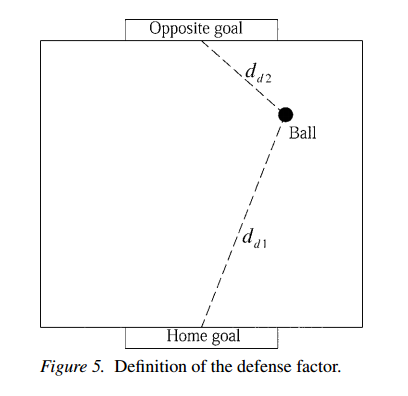
\includegraphics[width=0.7\linewidth]{defenseFactor}
	\caption{Defense Factor, image taken from \cite{wu2004fuzzy}}
	\label{fig:fig}
\end{figure}

\subsection{Competition Factor}
 the competition factor is defined as:
 
 \begin{equation}
 	f_{competition} = \phi_{dist}*e^{-\sigma_1*(d_1/d_2)} + (1 - \phi_{dist})*e^{-\sigma_2*(\theta_1/\theta_2)}
 \end{equation}

Where $d_{1}$ is the distance between the ball and the home robot, $d_{2}$ is the distance between the ball and the opponent robot, $\theta_{1}$ is the angle between the ball and the
home robot, $\theta_2$ is the angle between the ball and the opponent robot, $\sigma_1 = 3$ ,$\sigma_2 = 3$ and $\phi_{dist} = 0.7$.\\

The definition shows that the value of $f_{competition}$ varies between $0$ and $1$. $f_{competition} = 1$ indicates that the ball is very close to the home robot and the angle between the ball and the home robot is quite small, such that the home robot has a much better chance to control the ball than the opponent robot. On the other hand, if $f_{competition} = 0$, then the opponent robot will have an obvious advantage over the home robot.

\begin{figure}
	\centering
	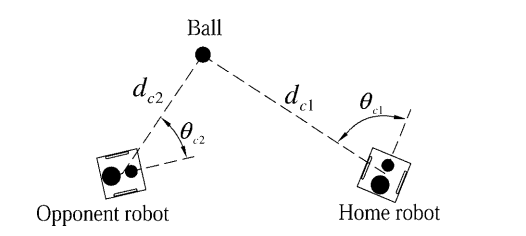
\includegraphics[width=0.7\linewidth]{competitionFactor}
	\caption{Competition Factor, image taken from \cite{wu2004fuzzy}}
	\label{fig:fig}
\end{figure}

\subsection{Angle factor}
The angle factor is defined as follows:

\begin{equation}
	f_{angle} = \frac{||y_b - y_r||}{\sqrt{(x_b - x_r)^2 + (y_b - y_r)^2}}
\end{equation}

where $(x_b, y_b)$ is the position of the ball and $(x_r, y_r)$ is the position of the home robot.
When $-90 \leq \sigma_a \leq 90$, it indicates that the ball is in front of the robot such that the robot can access the ball very easily. Otherwise, value of the angle factor is set to zero, since the ball is behind the robot. Therefore, the angle factor can be considered as a measure of the easiness of the robot to access the ball.

\begin{figure}
	\centering
	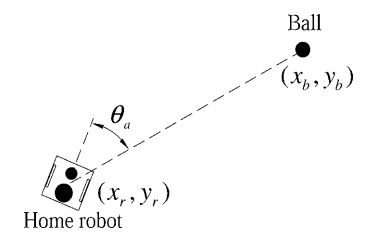
\includegraphics[width=0.7\linewidth]{angleFactor}
	\caption{Angle Factor, image taken from \cite{wu2004fuzzy}}
	\label{fig:fig}
\end{figure}

\subsection{Situation factor}

Factor that evaluate how crowded is a territory, the number of team mates  and opponents, in a territory, will be taken into account. The next formula describes this factor:

\begin{equation}
	f_{situation} = \frac{1}{(1 + e^{-\frac{C_{teams} - C_{opponents}}{\sigma}})}
\end{equation} 

Where $\sigma = 1.3$, $C_{team}$ the team mates on that territory and $C_{opponent}$ the opponents on it. If $f_{situation}=0$ means that the territory is too crowded with opponents and $f_{situation} = 1$ that the territory is not crowded enough.


\subsection{Coverage factor}

\begin{figure}
	\centering
	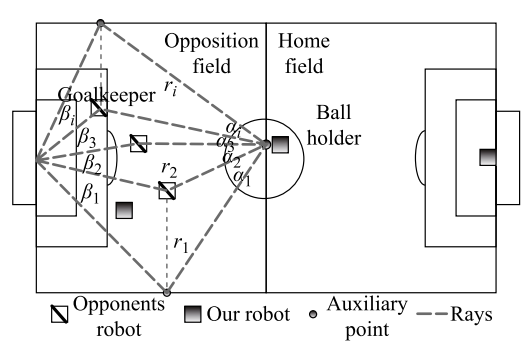
\includegraphics[width=0.7\linewidth]{covertureFactor}
	\caption{coverage Factor, image taken from \cite{shi2015research}}
	\label{fig:fig}
\end{figure}

First, auxiliary points are introduced to facilitate the modeling. Two auxiliary points are located in the upper and lower boundaries of the stadium and their x-coordinates are equal to the x-coordinates of the opponent robot that is closest to the upper and lower boundary.\\

Second, rays can be made from the ball center to each opponent robot center and auxiliary points, denote the angle between adjacent rays by $\alpha_i$. \\

Third, rays are be made from the midpoint of opponent goal line to each opponent robot centers and the auxiliary points, denote the angle between adjacent rays by $\beta_i$. \\

Denote the region between angle $\alpha_i$ and $\beta_i$ by $r_i$, $r_i = (\alpha_i, \beta_i)$. The larger the angle $\alpha_i + \beta_i$, the greater possibility for our ball holder to break through the opponent defense and threaten the goal in region $r_i$. Let the set $S$ comprised the angles $\alpha_i + \beta_j. S = {\alpha_i + \beta_i}, i = 0, 1, . . . , n$, and the difficulty to break through the opponents defense in region $r_i$ is inversely proportional to $S_i, S_i \in S $.\\

The coverage factor is defined as follows:

\begin{equation}
	f_{coverage} = 1 - e^{\frac{-r_i}{\sigma}}	
\end{equation}

Where $\sigma = 30$.  If $f_{coverage} = 0$ means that is impossible to approach the area, if $f_{coverage} = 1$ means the area is free.

\subsection{Penetration factor}

\begin{figure}
	\centering
	\includegraphics[width=0.7\linewidth]{penetrationFactor}
	\caption{Penetration Factor, image taken from \cite{shi2015research}}
	\label{fig:fig}
\end{figure}

The weakest opponent region $r_i$ can be calculated according to set $S , r_i \leftrightarrow max(S ) = max(\alpha_i + \beta_i)$. The bisector of angle $\alpha_i$ is $l_{\alpha i}$, and the bisector of angle $\beta_i$ is $l_{\beta i}$. Thus the line $l_{\alpha i}$ is considered to be the optimum offensive route of the main attacker in region $r_i$. \\

The penetration factor depends of the distant of the closest opponent robot to the line $l_{\alpha i}$, $d1$ in the figure, and to the main attacker. If these two distances are high the \textit{penetration factor} will also be high and the agent will dribble through the line $l_{\alpha i}$.\\

The distant of other assists robots to the line $l_{\alpha i}$, $d2$ in the figure, will be also taken into account with the distance $d3$ to form the \textit{Penetration assist factor}. If $d3$ is small and $d2$ is also small the main attacker will kick the ball in the $l_{\alpha i}$ direction. \\

The \textit{Penetration factor} and \textit{Penetration assist factor} functions are defined as follows:

\begin{equation}
	f_{penetration} = (1 - e^{\frac{-d_3}{\sigma_1}}) + 0.5*e^{\frac{-d_3}{\sigma_1}}*(1 - e^{\frac{d_1}{\sigma_2}}) 
\end{equation}

\begin{equation}
	f_{penetration} = 1 - \frac{1}{2} * e^{\frac{-d_3}{\sigma_1}} - \frac{1}{2} * e^{\frac{-d_3*\sigma_2 - d_1*\sigma_1}{\sigma_1 * \sigma_2}}
\end{equation}

\begin{equation}
	f_{penetrationAssist} = e^{\frac{-\sigma_3*d_3 - \sigma_1*d_2}{\sigma_1*\sigma_3}}
\end{equation}

Where:\\
 $\sigma_1 = 0.28$\\
 $\sigma_3 = 0.16= \sigma_2$
 
If $f_{penetration} = 1$ the player should dribble along $l_{\alpha}$, if $0$ should not. Also if $f_{penetrationAssist} = 1$ the player should kick the ball along $l_{\alpha}$, if $0$ should not.

\subsection{Shooting factor}

\begin{figure}
	\centering
	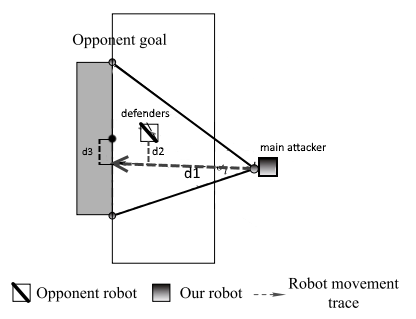
\includegraphics[width=0.7\linewidth]{shootingFactor}
	\caption{Shooting Factor}
	\label{fig:fig}
\end{figure}

The shooting factor depends of the distant $d_1$, $d_2$ and $d_3$. the smaller $d_1$ and $d_3$ are and the bigger $d_2$, the bigger this factor will be. The function $f_{shooting}$ is defined as follows:

\begin{equation}	
			f_{shooting} = (1-e^{\frac{-d_2}{\sigma_2}})*(e^{\frac{-d_1}{\sigma_1}} - \phi_{penalizacion} *(1 - e^{\frac{-d_3}{\sigma_3}}))
\end{equation}


\begin{equation} 
	f_{shooting} = e^{\frac{-d_1}{\sigma_1}}- e^{\frac{-d_1*\sigma_2 - d_2*\sigma_1}{\sigma_1*\sigma_2}} + \phi_{penalizacion} * (-1 -e^{\frac{-d_2}{\sigma_2}} + e^{\frac{-d_3}{\sigma_3}} - e^{\frac{-d_3*\sigma_3 - d_2*\sigma_2}{\sigma_3 * \sigma_2}})
\end{equation}

Where:\\
$\sigma_1 = 0.33$\\
$\sigma_2 = 0.16$\\
$\sigma_3 = 0.5$\\
$\phi_{penalizacion} = 0.4$

\begin{equation}
	f_{intercept} = e^{\frac{-d_1}{\sigma_1}} * e^{\frac{-d_2}{\sigma_2}} * e^{\frac{-d_3}{\sigma_3}}
\end{equation}
\begin{equation}
	f_{intercept} = e^{\frac{-d_1*\sigma_2*\sigma_3 -d_2*\sigma_1*\sigma_3 -d_3*\sigma_1*\sigma_2}{\sigma_1*\sigma_2*\sigma_3}}
\end{equation}

Where $\sigma_1 =  0.13$ , $\sigma_2 = 0.05$ and $\sigma_3 = 0.04$


If $f_{shooting} = 1$ the player should shoot thought $d_1$, if $0$ should not.\\
If $f_{intercept} = 1$ the player should intercept the ball  through $d_1$, if $0$ should not. 

\subsection{Keep Goal factor}

Use the distance of each player inside the goal area. The function decrements with the number of players in the area. The function is defined as follows:

\begin{equation}
	f_{keepGoal} = \frac{5 - \Sigma_i^5 e^{\frac{-d_i}{\sigma}}}{5} 
\end{equation}

Where $\sigma = 0.05$ and $d_i$ the distance of the player $i$ to the center of the goal. If $f_{keepGoal} = 0$ the goal is keep right , if $f_{keepGoal} = 1$ the goal need to be keep. 


%----------------------------------------------------------------------------------------
%	Actions & Thresholds
%----------------------------------------------------------------------------------------

\section{Actions and Thresholds}
In this section all the actions available to a player and their respective thresholds are described. Not all actions are available to a  certain player at any moment, for example for some actions like \textit{shoot} or \textit{pass} the player need to be in control of the ball. Only one action can be taken so when more than one thresholds are exceeded the one exceeded by most will be the one selected. The probability of selecting a undefined action $i$ for certain player $j$, is defined as follows:

\begin{equation}
	P_{action_i} = \frac{StimulusFunction(action_i)^{\sigma_1}}{ StimulusFunction(action_i)^{\sigma_1} + \varphi_j * \theta_j^{\sigma_2}}
\end{equation}

Where $\sigma_1$ and $\sigma_2$ are positive integer numbers, $\varphi_j$ is a number between [0,1] and $\theta_j$ is the threshold of the player $j$ for action $i$.

\subsection{With the ball}
These actions can only be made by the player who has the ball

\subsubsection{Advance}
Move a player forward, depends of: the situation factor of the next territory, the defense factor and the coverage factor. The stimuli function is defines as follows.

\begin{equation}
	S_{advance} = (\varphi_{sn} * f_{s}(next) + (1 - \varphi_{sn}) * f_{c}(player)) * (f_{d})
\end{equation}

Where:\\
$\varphi_{sn} = 0.30$ \\
$f_{s}(next)$ is the situation factor next territory \\
$f_{c}(player)$ is the coverage factor of the player\\
$f_{d}$ is  the defense factor.\\

If this action is taken the player will: dribble along the \textit{coverage factor} line.

\subsubsection{Pass to player}

\begin{figure}
	\centering
	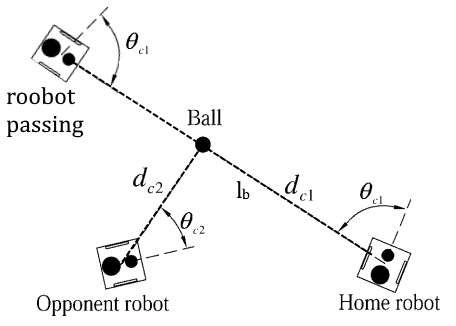
\includegraphics[width=0.7\linewidth]{passAction}
	\caption{Diagram for the pass action}
	\label{fig:fig}
\end{figure}

The player $i$ pass the ball to other player $j$, depends on the: coverage factor of player $i$ and player $j$, the distance between them, situation factor of player's $j$ area and the competition factor between the: player $j$ , he's nearest opponent and the middle of the line $l_a$ between player $j$ and player $i$. The stimuli function is defined as follows:

\begin{equation}
	S_{pass}(i) = \varphi_c * \frac{1}{(1 + e^{- \mu * \frac{f_{c}(j)}{f_{c}(i)} + \beta})} +  \varphi_d * e^{-\sigma * l_b} + \varphi_{cp} * f_{cp}(j,opp) + \varphi_{s} * f_{s}(j)
\end{equation}

Where:\\
$\varphi_c = 0.40$ \\
$f_{c}(j)$ is the coverage factor of player $j$.\\
$f_{c}(i)$ is the coverage factor of player $i$.\\
$\mu = 10$\\
$\beta = 15$\\
$\varphi_d = 0.25$ \\
$\sigma = 1.5$\\
$l_b$ is the line in the figure. \\
$\varphi_{cp} = 0.25$\\
$f_{cp}(j,opp)$ is the competition factor of $j$ and the opponent robot\\
$\varphi_{s} = 0.1$\\
$f_{s}(j)$ is the situation factor of $j$'s territory.\\

If this action is taken, the player $i$ pass the ball along $l_b$ to player $j$.

\subsubsection{Shoot}

The players shoot to the opponent's goal, depends on the: shooting, defense and penetration assist factors. The stimuli function is defined as follows:

\begin{equation}
	S_{shoot} = (1 - f_d) * (\varphi_s * f_s + (1 - \varphi_{s})* (1 - f_{pa}) )
\end{equation}

Where:\\
$f_d$ is the \textit{defense factor} \\
$f_s$ is the \textit{shooting factor} \\
$\varphi_{s} = 0.5$ \\
$f_{pa}$ is the \textit{penetration assist} factor\\

If this action is taken the player shoots along the \textit{shoot factor} $d_1$ line.

\subsubsection{Pass assist}

The players pass the ball to a team mate that is assisting , depends on the: shooting, defense and penetration assist factors. The stimuli function is defined as follows:

\begin{equation}
	S_{passAssist} = (1-f_d) * ((1-\varphi_s) * f_{pa} +  \varphi_{s})* (1-f_{s}) )
\end{equation}

Where:\\
$f_d$ is the \textit{defense factor} \\
$f_s$ is the \textit{shooting factor} \\
$\varphi_{s} = 0.5$ \\
$f_{pa}$ is the \textit{penetration assist} factor\\

If this action is taken the player pass the ball along the \textit{penetration factor} $l_\alpha$ line.

\subsubsection{Clear}
 The players clear the ball towards the opponent's field, depends on the: defense factor and situation factor. The stimuli function is defined as follows:
 
 \begin{equation}
	f_{clear} = f_d * ((1 - f_s(actual))
 \end{equation}

Where:\\
$f_d$ is the \textit{defense factor} \\
$f_{s}(actual)$ is the situation factor of the actual territory \\

If this action is taken, the player kick the ball along the middle of the bigger coverage area.

\subsection{Without the ball}
These actions can only be made by players who does not has the ball.

\subsubsection{Advance}
Move a player forward, depends of the: situation factor of the next territory, defense  and situation of the actual territory factors. The stimuli function is defines as follows.

\begin{equation}
	S_{advance} = \varphi_s * \frac{1}{(1 + e^{- \mu * \frac{f_{s}(next)}{f_{s}(actual)} + \beta})} + (1 - \varphi_s) * (1  - f_d)
\end{equation}

Where:\\
$\varphi_{s} = 0.40$ \\
$\mu = 7$\\
$\beta = 7$\\
$f_{s}(next)$ is the situation factor of the next territory \\
$f_{s}(actual)$ is the situation factor of the actual territory\\
$f_{d}$ is  the defense factor.\\

If this action is taken the player will advance to the less crowded area. To calculate this first a vector in opposite direction of every opponent, in the  field of view of the player, and with module proportional to the distance of the opponent to the player are calculated on the players position. Second the same is done for the team mates but in the same direction. Third all the vector are summed, if the direction on x axis is not pointing to the opponent's goal, the direction in that axis is inverted.

\begin{figure}
	\centering
	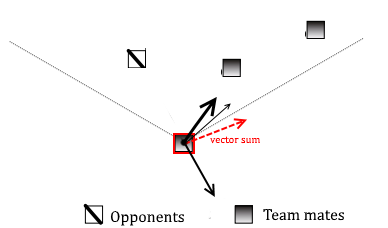
\includegraphics[width=0.7\linewidth]{lessCrowded}
	\caption{Diagram for the calculation of the less crowded area}
	\label{fig:fig}
\end{figure}

\subsubsection{Retreat}
Move a player back to it's field, depends of the: situation factor of the previous territory, defense  and situation of the actual territory factors. The stimuli function is defines as follows.

\begin{equation}
	S_{retreat} = \varphi_s * \frac{1}{(1 + e^{- \mu * \frac{f_{s}(actual)}{f_{s}(prev)} + \beta})} + (1 - \varphi_s) * (f_d)
\end{equation}

Where:\\
$\varphi_{s} = 0.40$ \\
$\mu = 7$\\
$\beta = 7$\\
$f_{s}(prev)$ is the situation factor of the previous territory \\
$f_{s}(actual)$ is the situation factor of the actual territory\\
$f_{d}$ is  the defense factor.\\

If this action is taken the player will retreat to the area with more opponents, this can be calculated the same way of the \textit{advance action} but swapping the opponents and the team mates. 

\subsubsection{Block player}

Move the player $i$ to block the opponent $j$, depends of the: \textit{j's} assist factor and penetration factor and competition factor between $i$ and $j$. The stimuli function is defined as follows:

\begin{equation}
	\varphi_c * (1 - f_{c}(i,j)) * ( \varphi_a * f_{a}(j) + (1-\varphi_a)*f_{p}(j))
\end{equation}

Where $\varphi_c = 1$, $f_c(i,j)$ is the competition factor between players $i$ and $j$, $\varphi_a = 0.4$, $f_a(j)$ is the assist factor of $j$ and $f_p(j)$ is the penetration factor of $j$. If this action is taken the player $i$ will go to block the player $j$.

\subsubsection{Cover goal}

Move the player to cover the goal, depends of the: defense and keep goal factors. The stimuli function is defined as follows:

\begin{equation}
	S_{coverGoal} = (1 - \varphi_d) * (f_d) + \varphi_d * f_k
\end{equation} 

Where:\\
$\varphi_d = 0.4$\\
$f_d$ is the defense factor\\
$f_k$ is the keep goal factor\\


If this action is taken the player moves to less crowded area of the goal.

\subsubsection{Intercepts}
Move the player to the intercept the ball, depends only of the \textit{intercept factor}. If this action is selected the player move to the nearest point of $d_1$.

\subsubsection{Assist}
Move the player trough the line $d_2$ in the \textit{penetration factor} figure. Depends of the defense and assist factor. The Stimuli function is defined as follow:

\begin{equation}
	S_{assist} = (1-f_d) * (f_{pa})
\end{equation}

If this action is taken, the player moves along $d_2$ line of the \textit{penetration factor} figure.

\subsubsection{Go to ball}

Move the player to the ball. depends only of the competition factor. If this action is taken the player moves along $d_1$ of the \textit{competition factor} figure.


%----------------------------------------------------------------------------------------
%	Positive Negative feedbak changing thresholds
%----------------------------------------------------------------------------------------

\section{Adjusting thresholds: Positive negative feedback}

In Bonabeu model \cite{bonabeau1997adaptive} the agent adjust their threshold when a task is performed, this approach need to be changed. Threshold will only be decreased for the action the players were doing if a beneficial action is done, for example retrieving the ball from the opponents, scoring , passing correctly ...etc. As Bonabeu proposed the  reinforcement will be:

\begin{equation}
	\theta_j = \theta_j - \epsilon(f_s,b_j)
\end{equation} 

\begin{equation}
	\epsilon(f_s,b_j) = valor(b_j) + (\frac{1}{1 + e^{-\sigma * f_s + \alpha}} - 0.5)*valor(b_j)
\end{equation}

Where $\theta_j$ is the threshold of a player to action $j$ ,which was the one that the player did when the beneficial action happened, $\epsilon(f_s,j)$ is a function that depends of the: \textit{score factor} and the beneficial action that triggers the update $b_j$.$\sigma = 8$ , $\alpha = 4$ and $valor(b_j)$ is the ones in the table below.\\

\begin{center}
\begin{tabular}{ |c|c| } 
 \hline
 action & value \\
 \hline\hline
 score & 0.2\\ 
 retrieve ball & 0.2\\
 intercepts ball & 0.2\\
 correct pass & 0.1\\
 player with ball enter opponents area & 0.1\\
 ball kick off our area & 0.1\\
 player with ball exit our field & 0.1 \\
 ball exit our field & 0.05\\   
 \hline
\end{tabular}
\end{center}

All the threshold will be restored to normal as time goes by, until a maximum is reach, so if not good action are happening the player forgets his bias. This forget function is as follows:

\begin{equation}
	\theta_j = \theta_j + \phi(f_s,f_t)
\end{equation}

\begin{equation}
	\phi(f_s, f_t) = \mu - (0.5 * f_s * \mu + f_t *(\frac{1}{1 + e^{-\sigma * f_s + \alpha}} - 0.5)*\mu)
\end{equation}

Where $\theta_j$ is the threshold of a player to action $j$ and $\phi(f_s,f_t)$ is a function that depends of the: \textit{score factor}, \textit{time factor}. $\sigma = 8$ , $\alpha = 4$. 

%----------------------------------------------------------------------------------------
%	Results
%----------------------------------------------------------------------------------------

\section{Results}

%----------------------------------------------------------------------------------------
%	Conclusions future work
%----------------------------------------------------------------------------------------

\section{Conclusions and future work}

%----------------------------------------------------------------------------------------
%	BIBLIOGRAPHY
%----------------------------------------------------------------------------------------

\renewcommand{\refname}{\spacedlowsmallcaps{References}} % For modifying the bibliography heading

\bibliographystyle{unsrt}

\bibliography{sample} % The file containing the bibliography

%----------------------------------------------------------------------------------------

\end{document}
